\documentclass{article}
\usepackage{tikz}
\usepackage{amsmath}
\usepackage{graphicx}

\usetikzlibrary{calc, patterns}

\title{Double Pendulum on a Cart}
\author{Kanish H R}
\date{April 2026}

\begin{document}
\maketitle

\begin{center}
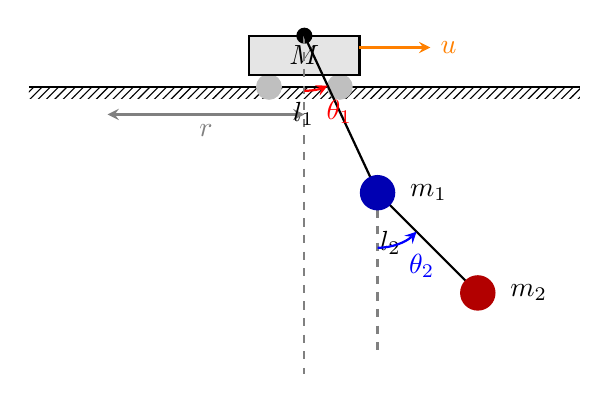
\begin{tikzpicture}[>=stealth, thick]

    % Parameters
    \def\lOne{2.2}
    \def\lTwo{1.8}
    \def\tOne{25}
    \def\tTwo{45}
    \def\cartW{1.4}
    \def\cartH{0.5}
    \def\cartX{0}

    % Ground / track
    \fill[pattern=north east lines] (-3.5, -0.35) rectangle (3.5, -0.5);
    \draw[thick] (-3.5, -0.35) -- (3.5, -0.35);

    % Cart wheels
    \filldraw[gray!50] (\cartX-0.45, -0.35) circle (0.15);
    \filldraw[gray!50] (\cartX+0.45, -0.35) circle (0.15);

    % Cart body
    \draw[thick, fill=gray!20]
        (\cartX-\cartW/2, -0.2) rectangle (\cartX+\cartW/2, \cartH-0.2);
    \node at (\cartX, 0.05) {$M$};

    % Cart position arrow
    \draw[<->, gray] (-2.5, -0.7) -- (\cartX, -0.7)
        node[midway, below] {$r$};

    % Pivot at top of cart
    \coordinate (O) at (\cartX, \cartH-0.2);
    \filldraw[black] (O) circle (2.5pt);

    % Pendulum coordinates
    \coordinate (M1) at (
        {\cartX + \lOne*sin(\tOne)},
        {\cartH-0.2 - \lOne*cos(\tOne)}
    );
    \coordinate (M2) at (
        {\cartX + \lOne*sin(\tOne) + \lTwo*sin(\tTwo)},
        {\cartH-0.2 - \lOne*cos(\tOne) - \lTwo*cos(\tTwo)}
    );

    % Dashed vertical references
    \draw[dashed, gray] (O)  -- ++(0, {-\lOne - \lTwo - 0.3});
    \draw[dashed, gray] (M1) -- ++(0, {-\lTwo - 0.3});

    % Rods
    \draw[thick] (O)  -- (M1);
    \draw[thick] (M1) -- (M2);

    % Masses
    \filldraw[blue!70!black] (M1) circle (6pt);
    \filldraw[red!70!black]  (M2) circle (6pt);

    % Mass labels
    \node[right=8pt] at (M1) {$m_1$};
    \node[right=8pt] at (M2) {$m_2$};

    % Length labels
    \node[left=6pt] at ($(O)!0.5!(M1)$)  {$l_1$};
    \node[left=6pt] at ($(M1)!0.5!(M2)$) {$l_2$};

    % Theta1 arc
    \draw[->, red] ({\cartX}, {\cartH-0.2-0.7})
        arc[start angle=270, delta angle=\tOne, radius=0.7]
        node[midway, below right] {$\theta_1$};

    % Theta2 arc
    \draw[->, blue] ($(M1) + (0, -0.7)$)
        arc[start angle=270, delta angle=\tTwo, radius=0.7]
        node[midway, below right] {$\theta_2$};

    % Control force arrow
    \draw[->, thick, orange] (\cartX+\cartW/2, 0.15) -- ++(0.9, 0)
        node[right] {$u$};

\end{tikzpicture}
\end{center}

\section*{Cart + Double Pendulum: Lagrangian Derivation}

\subsection*{Generalised Coordinates}
The system has three degrees of freedom: cart position $r$, and pendulum angles $\theta_1$, $\theta_2$.

\subsection*{Position Vectors}
\begin{align}
    \vec{x}_\text{cart} &= (r,\ 0) \\
    \vec{x}_1 &= (r + l_1\sin\theta_1,\ {-l_1\cos\theta_1}) \\
    \vec{x}_2 &= (r + l_1\sin\theta_1 + l_2\sin\theta_2,\ {-(l_1\cos\theta_1 + l_2\cos\theta_2)})
\end{align}

\subsection*{Velocity magnitudes squared}
\begin{align}
    |\dot{\vec{x}}_1|^2 &= \dot{r}^2 + 2\dot{r}\,l_1\cos\theta_1\,\dot{\theta}_1 + l_1^2\dot{\theta}_1^2 \\
    |\dot{\vec{x}}_2|^2 &= \dot{r}^2 + l_1^2\dot{\theta}_1^2 + l_2^2\dot{\theta}_2^2
        + 2\dot{r}\,l_1\cos\theta_1\,\dot{\theta}_1
        + 2\dot{r}\,l_2\cos\theta_2\,\dot{\theta}_2
        + 2l_1 l_2\cos(\theta_2-\theta_1)\,\dot{\theta}_1\dot{\theta}_2
\end{align}

\subsection*{Kinetic and Potential Energy}
\begin{align}
    T &= \tfrac{1}{2}(M+m_1+m_2)\dot{r}^2
       + \tfrac{1}{2}(m_1+m_2)l_1^2\dot{\theta}_1^2
       + \tfrac{1}{2}m_2 l_2^2\dot{\theta}_2^2 \notag \\
      &\quad + (m_1+m_2)l_1\cos\theta_1\,\dot{r}\dot{\theta}_1
       + m_2 l_2\cos\theta_2\,\dot{r}\dot{\theta}_2
       + m_2 l_1 l_2\cos(\theta_2-\theta_1)\,\dot{\theta}_1\dot{\theta}_2 \\[6pt]
    V &= -(m_1+m_2)g l_1\cos\theta_1 - m_2 g l_2\cos\theta_2
\end{align}

\subsection*{Euler-Lagrange Equations in Matrix Form}

Applying $\dfrac{d}{dt}\!\left(\dfrac{\partial L}{\partial \dot{q}_i}\right) = \dfrac{\partial L}{\partial q_i}$
for $q = (r, \theta_1, \theta_2)$ yields the coupled system
$\mathbf{M}(\theta)\,\ddot{\mathbf{q}} = \mathbf{f}(\theta, \dot{\theta})$:

\begin{equation}
\underbrace{\begin{bmatrix}
    M+m_1+m_2 & (m_1+m_2)l_1\cos\theta_1 & m_2 l_2\cos\theta_2 \\
    (m_1+m_2)l_1\cos\theta_1 & (m_1+m_2)l_1^2 & m_2 l_1 l_2\cos(\theta_2-\theta_1) \\
    m_2 l_2\cos\theta_2 & m_2 l_1 l_2\cos(\theta_2-\theta_1) & m_2 l_2^2
\end{bmatrix}}_{\mathbf{M}(\theta)}
\begin{bmatrix} \ddot{r} \\ \ddot{\theta}_1 \\ \ddot{\theta}_2 \end{bmatrix}
=
\begin{bmatrix} f_1 \\ f_2 \\ f_3 \end{bmatrix}
\end{equation}

where
\begin{align}
    f_1 &= (m_1+m_2)l_1\sin\theta_1\,\dot{\theta}_1^2
           + m_2 l_2\sin\theta_2\,\dot{\theta}_2^2 + u \\
    f_2 &= -m_2 l_1 l_2\sin(\theta_1-\theta_2)\,\dot{\theta}_2^2
           - (m_1+m_2)g l_1\sin\theta_1 \\
    f_3 &= \phantom{-}m_2 l_1 l_2\sin(\theta_1-\theta_2)\,\dot{\theta}_1^2
           - m_2 g l_2\sin\theta_2
\end{align}

\subsection*{Solution via Cramer's Rule}

Let $D = \det\mathbf{M}(\theta)$ and $\mathbf{M}^{(i)}$ denote $\mathbf{M}$ with column $i$ replaced by $\mathbf{f}$. Then:

\begin{equation}
    \ddot{r} = \frac{\det\mathbf{M}^{(1)}}{D}, \qquad
    \ddot{\theta}_1 = \frac{\det\mathbf{M}^{(2)}}{D}, \qquad
    \ddot{\theta}_2 = \frac{\det\mathbf{M}^{(3)}}{D}
\end{equation}

\end{document}
